\documentclass[a4paper,12pt]{article}
\usepackage{geometry}
\usepackage{enumitem}
\usepackage{fancyhdr}
\usepackage{xcolor}
\usepackage{sectsty}
\usepackage{multicol}
\usepackage{graphicx}
\usepackage{amsmath}
\usepackage{float}
\def\inputGnumericTable{}
\usepackage[latin1]{inputenc}
\usepackage{fullpage}
\usepackage{color}
\usepackage{array}
\usepackage{longtable}
\usepackage{calc}
\usepackage{multirow}
\usepackage{hhline}
\usepackage{ifthen}
\geometry{top=1in, bottom=1.5cm, left=1.5cm, right=1.5cm}    
\pagestyle{empty}
\sectionfont{\color{blue}}

\begin{document}

\thispagestyle{fancy}
\fancyhf{}
\fancyhead[L]{
    
\includegraphics[width=8cm, height=1.7cm]{IIITB-COMET-Logo.png}
}
\fancyhead[R]{
    Name: N.Srinivas \\
    Batch: COMETFWC036 \\
    Date: 10 September 2025
}
\renewcommand{\headrulewidth}{0pt}
\fancyfoot[C]{\thepage}

\vspace*{1cm}
\begin{center}
    {\LARGE \textbf{\textcolor{blue}{GATE 2010 CS, $31^{th}$ Question Analysis}}}
\end{center}
\section*{Q.31}
What is the boolean expression for the output $f$ of the combinational logic circuit of NOR gates given below?

\begin{center}
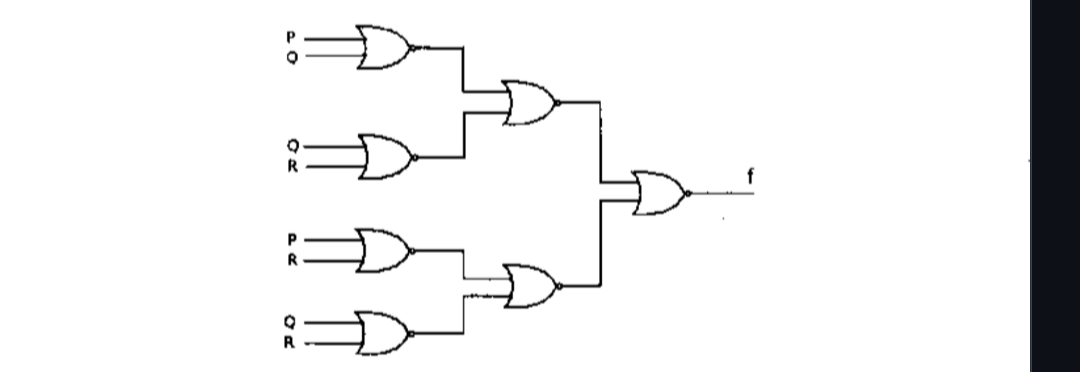
\includegraphics[width=0.7\textwidth]{Circuit.jpg}
\end{center}

\subsection*{Solution}

Each gate in the circuit is a NOR gate, which performs the operation:
$
A \downarrow B = \overline{A + B}
$

\begin{itemize}
    \item Gate A: $A = \overline{P + Q}$
    \item Gate B: $B = \overline{Q + R}$
    \item Gate C: $C = \overline{A + B} = \overline{\overline{P + Q} + \overline{Q + R}}$
    \item Gate D: $D = \overline{P + R}$
    \item Gate E: $E = \overline{Q + R}$
    \item Gate F: $F = \overline{D + E} = \overline{\overline{P + R} + \overline{Q + R}}$
    \item Final Output: 
    $
    f = \overline{C + F} = \overline{ \overline{ \overline{P + Q} + \overline{Q + R} } + \overline{ \overline{P + R} + \overline{Q + R} } }
    $
\end{itemize}

\subsection*{Truth Table}

\begin{center}
\begin{tabular}{|c|c|c|c|}
\hline
P & Q & R & $f = \overline{Q + R}$ \\
\hline
0 & 0 & 0 & 1 \\
0 & 0 & 1 & 0 \\
0 & 1 & 0 & 0 \\
0 & 1 & 1 & 0 \\
1 & 0 & 0 & 1 \\
1 & 0 & 1 & 0 \\
1 & 1 & 0 & 0 \\
1 & 1 & 1 & 0 \\
\hline
\end{tabular}
\end{center}
\section*{\textbf{Hardware Implementation}}
The above problem is implemented and tested in hardware using Arduino UNO board. Here we implemented a FSM using the 7474 IC and blinked the LED as per truth table and verified the expression.
\section*{Required Components \& Pin Connections}
\begin{center}
\begin{minipage}{0.45\textwidth}
\begin{table}[H]
\centering
\begin{tabular}{|c|l|}
\hline
\textbf{S.No} & \textbf{Component} \\ \hline
1 & Arduino Uno Board \\
2 & Breadboard \\
3 & LEDs (1) \\
4 & 7447 IC (1) \\
5 & Seven segment (1) \\
6 & Resistors: 220$\Omega$ (2) \\
7 & Jumper Wires \\
8 & USB Cable \\
\hline
\end{tabular}
\end{table}
\end{minipage}
\hspace{0.05\textwidth}
\begin{minipage}{0.45\textwidth}
\begin{table}[H]
\centering
\begin{tabular}{|c|c|}
\hline
\textbf{Component} & \textbf{Arduino Pin} \\ \hline
Input P  & Digital 2 \\
Input Q  & Digital 3 \\
Input R  & Digital 4 \\
Output sevensegment(a) & 7447(a)\\
Output sevensegment(b) & 7447(b)\\
Output sevensegment(c) & 7447(c)\\
Output sevensegment(d) & 7447(d)\\
Output sevensegment(e) & 7447(e)\\
Output sevensegment(f) & 7447(f)\\
Output sevensegment(g) & 7447(g)\\
Output F (LED) & Digital 5 \\
GND & GND \\
VCC & 5V \\
\hline
\end{tabular}
\end{table}
\end{minipage}
\end{center}
\section*{Code Uploading Steps}
\begin{enumerate}
	\item Create a avr-gcc  project
	\item Write The code in main.c in src
	\item Run the PIO project with command "make hex". It will compile the code and creates .hex file
	\item Copy the .hex file to ArduinoDriod folder
	\item connect the Arduino UNO to mobile with OTG cable
	\item Upload the hex file using "upload precomplied" option
	\item Observe the ouput and verify the expression
\end{enumerate}

\subsection*{Answer:}

$
\boxed{f = \overline{Q + R}}
$

Correct option: \textbf{(A)}

\end{document}

